%\svnInfo $Id: Ch3_2017.tex 65 2017-08-14 19:39:16Z Georg Lindgren $ 
%$
%
\chapter[Empirical wave characteristics]{%
Empirical wave characteristics}
\label{cha:distr-appar-wave-data}\label{cha:3}

%=====================
%---------------------
%=====================
One of the unique capabilities of \progname{} is the treatment of
the statistical properties of wave characteristic. This, and the next chapter,
describe how to extract information on distributions of observables like
wave period, wave length, crest height, etc, either directly from data, or
from empirically fitted approximative models, or, in the next chapter, by means
of exact statistical distributions, numerically computed from a spectral model.

We first define the different wave characteristics commonly used in
oceanographic engineering and science, and present the \progname{} routines
for handling them. Then we compare the empirical findings with some
approximative representations of the statistical distributions, based
on empirical parameters from observed sea states. The code for the examples
are found in the m-file \verb+Chapter3.m+, and it takes a few seconds to run.

\section{Introduction}
\index[xentr]{wave characteristics|(}
\subsection{The Gaussian paradigm - linear wave theory}\label{ss:gaussianparadigm}
\index{linear wave theory}
In the previous chapter we discussed modelling of random functions by
means of Fourier methods. The signal was represented as a sum of
independent random cosine functions with random amplitudes and phases. In linear
wave theory those cosine functions are waves travelling in water. Waves
with different frequencies have different speeds, defined by the
dispersion relation. \index[xentr]{dispersion relation}
This property causes the characteristic
irregularity of the sea surface. Even if it were possible to arrange a very
particular combination of phases and amplitudes, so that the signal
looks, for example, like a saw blade, it will, after a while, change
shape totally. The phases will be almost independent and the sea would
again look like a Gaussian random process. On the other hand an
observer clearly can identify moving  sea waves. The shape of those
waves, which are often called the
{\sl apparent  waves},\index[xentr]{apparent!wave}
since theoretically, those are not mathematical waves, but are constantly
changing up to the moment when they disappear.

The wave action on marine structures is often modelled using linear filters.
Then the sea spectrum, together with the filter frequency function,
gives a complete characterization of the response
of the structure. However, often such models are too simplistic
and non-linearities have to be considered to allow more complex responses.
Then one may not wish to perform a complicated numerical
analysis to derive the complete response but is willing to accept
the simplification that the response is proportional to the waves.
One may also wish to identify some properties of waves that are dangerous
in some way for the particular ocean operation.
Also the apparent waves themselves can be the reason for non-linear response.
For example, for waves with crests higher than some
threshold, water may fill a structure and change its dynamical properties.
The combined effect of apparent waves, often described by their
height and wave period, is therefore important in ocean engineering.
These aspects are discussed in more detail in
the textbook \cite{Ochi1998Ocean}.

The apparent waves will be described by some geometric properties,
called wave characteristics, while frequencies of
occurrences of waves with specified characteristics will be treated in the
statistical sense and described by a probability distribution. Such
distributions can then be used to estimate the frequency of occurrences
of some events important in the design of floating marine systems,
e.g.\ wave breaking, slamming, ringing, etc.

\subsection{Wave characteristics in time and space}
The wave surface is clearly a two-dimensional phenomenon that changes
with time and its study naturally deals with moving two-dimensional
objects (surfaces). Theoretical studies of random surfaces are the 
subject of ongoing research, for example,
\cite{AzaisWschebor2009,Mercardier2006},
for general studies of Gaussian random surfaces, 
\cite{Aberg2007diss,AbergRychlikLeadbetter2008,BaxevaniEtal2003Velocities,
BaxevaniRychlik2006,PodgorskiEtal2000Statistics,Sjo2000Crossing,Sjo2001Simultaneous}, 
for space-time related wave results, and \cite{PodgorskiRychlik2016SizeOfWaves} 
for wave geometry. 
Related results for Lagrange models are found in
\cite{AbergLindgren2008,Lindgren2006,Lindgren2009,Lindgren2010a,
LindgrenAberg2009,Lindgrenetal2010}.

At present, there are only few programs in \progname{} that
handle the space-time relations of waves, and hence in this tutorial we limit 
the presentation to simpler cases of waves in one-dimensional \index[xentr]{Lagrange waves}
records.\footnote{The Lagrange module in \progname{} contains special  
space-time routines for (Gaussian and) non-Gaussian waves; a tutorial is included in that module.} 
By this we mean the apparent waves extracted from functions
(measured signals) with one-dimensional parameter, either in time or in
space. These functions can be extracted from a photograph of the sea
surface as, for example, the {\it instantaneous profile} along a line
in some fixed horizontal direction on the sea, or they can be obtained
directly as a {\em record taken in time at a fixed position in space}
as by means of a wave pole or distance meter.  The
{\em encountered sea},\index[xentr]{encountered sea}
another important one-dimensional record, can be collected
by means of a ship-borne wave recorder moving across the random sea.

To analyze collected wave data we need natural and operational
definitions of an individual wave, its period, height, steepness, and
possibly some other meaningful characteristics. There are several
possible definitions of apparent wave, and here we shall concentrate
mostly on zero down-crossing waves. Namely, the
{\em apparent individual wave}
at a fixed time or position is defined as the part
of the record that falls between two consecutive down-crossings of the
zero seaway level (the latter often more descriptively referred to as
the still water level).  For individual waves one can consider various
natural characteristics, among them {\em apparent periods}  and
{\em apparent heights (amplitudes)}. The pictorial definitions of these
characteristics are given in \index[xentr]{apparent!period}
Figure~\ref{fig:wavpar}. \index[xentr]{apparent!height}
\begin{figure}[tbh]
\centering
  %\includegraphics[width=0.6\textwidth,angle=-90]{005f_wvp}
  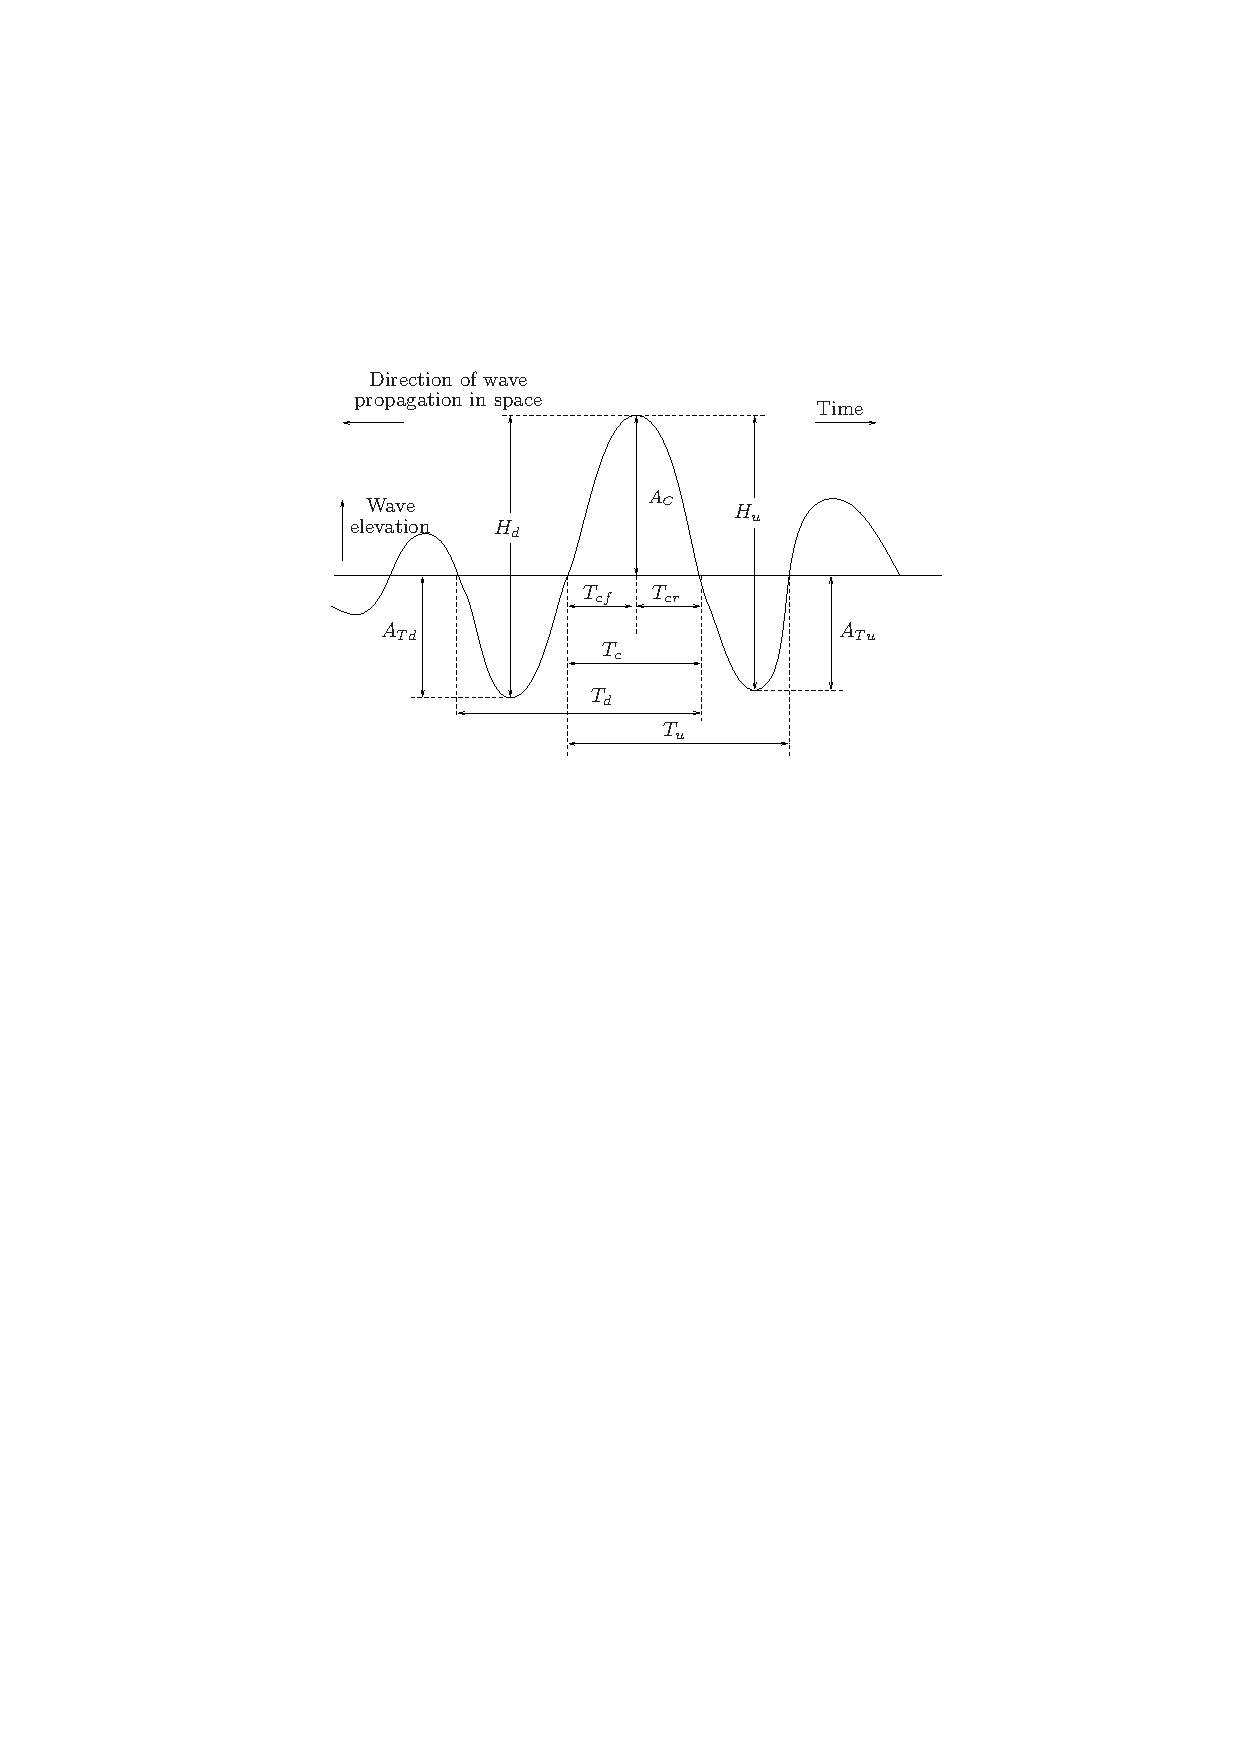
\includegraphics[width=0.7\textwidth,angle=0]{waveparamNew}
\vspace{-3mm}
  \caption[Definition of wave parameters]
{Definition of wave parameters. The notation for the parameters
used in our examples are given in Table~\ref{tab3_1} at the end of this chapter.}
  \label{fig:wavpar}
  \end{figure}

The definitions of the most common wave characteristics are given in
Table~\ref{tab3_1}. In the \progname{} toolbox, the most important can be
retrieved by the help commands for {\tt wavedef}, {\tt perioddef},
{\tt ampdef}, and {\tt crossdef}, producing the output in
Section~\ref{sec:WAFOcharacteristics}.
\index[xcmds]{{\tt wavedef}}
\index[xcmds]{{\tt perioddef}}
\index[xcmds]{{\tt ampdef}}
\index[xcmds]{{\tt crossdef}}

Having precisely defined the characteristics of interest, one can
extract their frequency (empirical) distributions from a typical
sufficiently long record.  For example, measurements of the apparent
period and height of waves could be taken over a long
observation interval to form an empirical two-dimensional
distribution. This distribution will represent some aspects of a given
sea surface. Clearly, because of the irregularity of the sea,
empirical frequencies will vary from record to record. However if the
sea is in ``steady'' condition, which corresponds mathematically to
the assumption that the observed random field is stationary and
ergodic, their variability will be insignificant for sufficiently
large records. Such limiting distributions (limiting with respect to
observation time, for records measured in time, increasing without
bound) are termed the
{\em long-run distributions}. \index[xentr]{long-run distribution}
Obviously, in a real 
sea we seldom have a so long period of "steady" conditions that the
limiting distribution will be reached. On average, one may observe
400-500 waves per hour of measurements, while the stationary
conditions may last from 20 minutes to only a few hours.

Despite of this, a fact that makes these long-run distributions particularly
attractive is that they give probabilities of occurrence of waves that
may not be observed in the short records but still are possible. Hence,
one can estimate the intensity of occurrence of waves with special
properties and then extrapolate beyond the observed types of waves.
What we shall be concerned with next is how to compute such
distributional properties.

In the following we shall consider three different ways to
obtain the wave characteristic probability densities (or
distributions):

\begin{itemize}
\item
To fit an empirical distribution to observed (or simulated) data in
some parametric family of densities, and then relate the estimated
parameters to some observed wave climate described by means of
significant wave heigh and wave period. Algorithms to extract
waves, estimate the densities and compute some simple statistics will
be presented here in Chapter~\ref{cha:3}

\item
To simplify the model for the sea surface to such a degree that
explicit computation of wave characteristic densities (in the
simplified model) is possible. Some examples of proposed models from
the literature will also be given in this chapter.

\item
To exactly compute the statistical distribution from the mathematical form of a
random seaway. This requires computation of infinite
dimensional integrals and expectations that have to be
computed numerically. \progname{} contains efficient numerical
algorithms to compute these integrals, algorithms which do not require
any particular form of the sea surface spectrum.
The method are illustrated in Chapter~\ref{cha:4}
on period, wavelength, and amplitude
distributions, for many standard types of wave
spectra.
\end{itemize}

\section{Estimation of wave characteristics from data}
\label{sec:estim-wave-char}
\index[xentr]{wave characteristics!estimation from data|(}

In this section we shall extract the wave characteristics from a
measured signal and then use non-parametric statistical methods
to describe the data, i.e.\ empirical distributions, histograms,
and kernel estimators.
(In the last chapter of this tutorial  we present some statistical
tools to fit parametric models; for kernel estimators, see Appendix~\ref{cha:KDE}.)

It is generally to be advised that, before analyzing sea wave
characteristics, one should check the quality of the data by inspection
and by the routine \verb+findoutliers+ used in Section~\ref{sect2.1}.
Then, one usually should remove any present trend
from the data. Trends could be due to tides or atmospheric pressure
variations that affect the mean level. De-trending can be done using the
\progname{} functions {\tt detrend}\index[xcmds]{{\tt detrend}} or
{\tt detrendma}\index[xcmds]{{\tt detrendma}}.
\index[xcmds]{{\tt findoutliers}}

\subsection{Wave period}
\index[xentr]{wave distributions!estimation of densities!wave period}
\begin{cex}{Ex_sea_statistics}
We now continue the analysis of the shallow water waves in {\tt sea.dat} that 
we started on page~\pageref{pageseadat}. 
We begin with extracting the apparent waves
\index[xentr]{apparent wave!extraction of} and record their period.
The signal  {\tt sea.dat} is recorded at 4~Hz sampling frequency.
One of the possible definitions of period is the time between the
consecutive wave crests. For this particular variable it may be
convenient to have a higher resolution than 4~Hz and hence we shall
interpolate the signal to a denser grid. This will be obtained by giving
an appropriate value to the variable {\tt rate} which can be used as input
to the \progname{} routine \verb+dat2wa+\index[xcmds]{{\tt dat2wa}}.
The following \index[xcmds]{{\tt rate}}
code will return crest2crest wave periods $T_{cc}$ in the variable
{\tt Tcrcr} and return the crest period $T_c$ in {\tt Tc}, i.e.\ the time from
up-crossings to the following down-crossing.
{\small\begin{verbatim}
      xx = load('sea.dat');
      xx(:,2) = detrend(xx(:,2));
      rate = 8;
      Tcrcr = dat2wa(xx,0,'c2c','tw',rate);
      Tc = dat2wa(xx,0,'u2d','tw',rate);
\end{verbatim}}

Next we shall use a kernel density estimator
(KDE) \index[xcmds]{{\tt kde}}
to estimate the probability density function (pdf)
of the crest period and compare the resulting pdf with a
histogram of the observed periods stored in {\tt Tc}.
In order to define a suitable scale for the density we first compute the
mean and maximum of the observed \index[xcmds]{{\tt kdeoptse}}
crest periods.
{\small\begin{verbatim}
      mean(Tc)
      max(Tc)
      t = linspace(0.01,8,200);
      kopt = kdeoptset('L2',0);
      ftc1 = kde(Tc,kopt,t);
      pdfplot(ftc1), hold on
      histgrm(Tc,[],[],1)
      axis([0 8 0 0.5])
\end{verbatim}}\index[xcmds]{{\tt kde}}
\noindent
(The parameter {\tt L2=0}  is used internally in  {\tt kde}, and
causes a logarithmic transformation of the data to ensure that the density
is zero for negative values. Run \verb+help kdeoptset+ to see the definition.)

\begin{figure}
\centering
  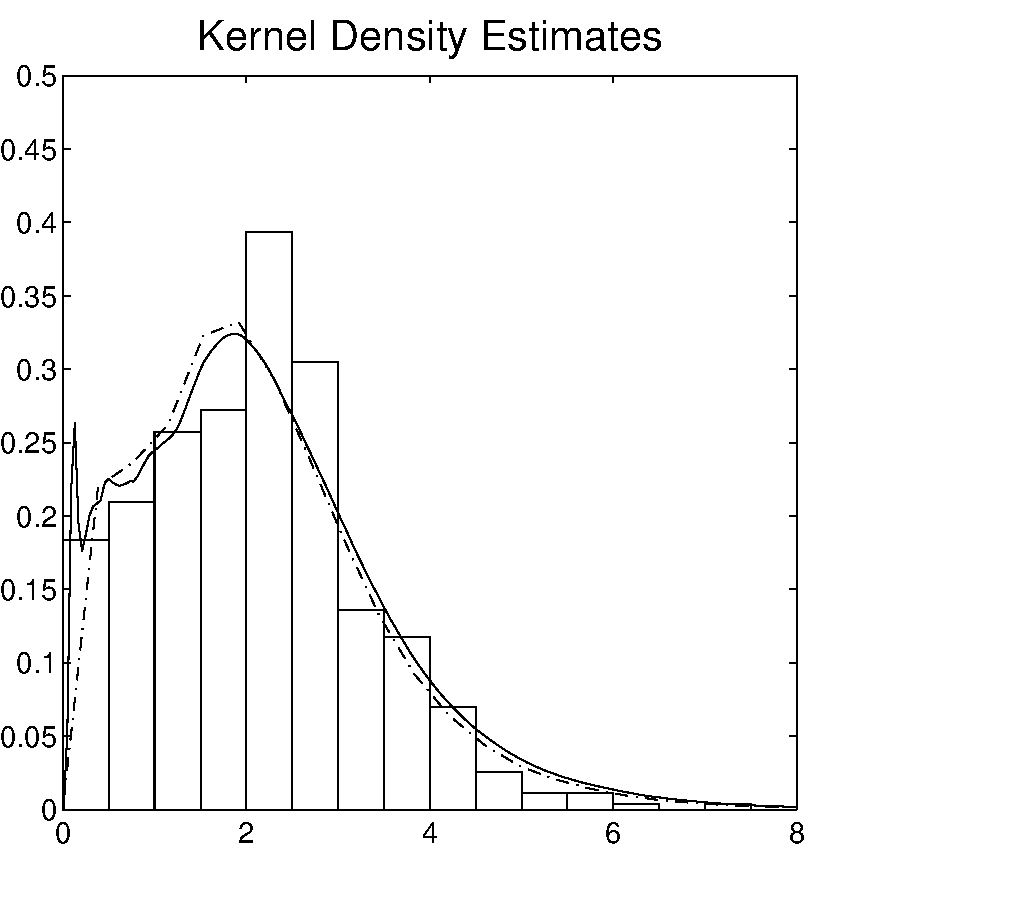
\includegraphics[width=\narrowfigwidth]{fig7_kde_tc}
\vspace{-3mm}
  \caption[Kernel estimate of the crest period density]{
Kernel estimate of crest period density observed in {\tt sea.dat};
solid line: full KDE, dash dotted line: binned KDE,
compared with histogram of the data.
}
  \label{fig7_kde_tc}
\end{figure}
In Figure~\ref{fig7_kde_tc} we can see that many short
waves have been recorded (due to relatively high sampling frequency).
The kernel estimate will be compared with the theoretically
computed density in Figure~\ref{fig73} in Chapter~\ref{cha:4},
%page~\pageref{page:Ex7a}.
page~\pageref{fig73}.
\end{cex}

\begin{remark} Note that the program {\tt kde}
can be quite slow for large data sets. If a faster estimate of the
density for the observations is preferred one can use
{\tt kdebin}\index[xcmds]{{\tt kdebin}},
which is an approximation to the true kernel density estimator. An
important input parameter in the program, that defines the degree of
approximation, is {\tt inc} which should be given a value between 100 and
500. (A value of {\tt inc} below 50 gives fast execution times
but can lead to inaccurate results.)
{\small\begin{verbatim}
      kopt.inc = 128;
      ftc2 = kdebin(Tc,kopt); pdfplot(ftc2,'-.')
      title('Kernel Density Estimates'), hold off
\end{verbatim}}
\noindent The result is in
Figure~\ref{fig7_kde_tc}  \index[xcmds]{{\tt inc}}
\end{remark}

\subsection{Extreme waves -- model check}
We turn now to joint wave characteristics, e.g.\ the joint density of
half period and crest height {\tt (Tc,Ac)}, or waveheight and steepness
{\tt (Ac,S)}. The program {\tt dat2steep} identifies apparent waves and 
for each wave gives several wave characteristics
(use the help function on {\tt dat2steep} for
a list of computed variables). \index[xcmds]{{\tt dat2steep}}
We begin by examining profiles of waves having some special property,
e.g.\ with high crests, or that are extremely steep.

\begin{cex}{Ex_sea_statistics}
The following code  finds a sequence of waves in {\tt sea.dat} and extracts 
their characteristics:
{\small\begin{verbatim}
      method = 0; rate = 8;
      [S, H, Ac, At, Tcf, Tcb, z_ind, yn] = ...
             dat2steep(xx,rate,method);
\end{verbatim}}

The first preliminary analysis of the data is to find the individual waves
which are extreme by some specified criterion, e.g.\ the steepest or the
highest waves, etc. To do such an analysis one can use the function
{\tt spwaveplot(xx,ind)}\index[xcmds]{{\tt spwaveplot}}, which plots
waves in {\tt xx} that are selected by the index variable {\tt ind}.
For example, let us look at the highest and the steepest waves.
{\small\begin{verbatim}
      [Smax indS] = max(S)
      [Amax indA] = max(Ac)
      spwaveplot(yn,[indA indS],'k.')
\end{verbatim}}

The two waves are shown in Figure~\ref{fig_c_wave}(a). The  shape of
the biggest wave reminds of the so called "extreme" waves.
In the following we shall examine whether this particular shape contradicts
the assumption of a transformed Gaussian model for the sea.

This is done as follows. First we find the wave with the highest crest.
Then we mark all positive values in that wave as missing.
Next we reconstruct the signal, assuming the Gaussian model is valid,
and compare the profile of the reconstructed wave with the actual
measurements.
Confidence bands for the reconstruction will also be plotted.
In the previous chapter we have already used the program
{\tt reconstruct}, \index[xcmds]{{\tt reconstruct}} and here
we shall need some additional output from that function, to be used to
compute and plot the confidence bands.
{\small\begin{verbatim}
      inds1 = (5965:5974)'; Nsim = 10;
      [y1, grec1, g2, test, tobs, mu1o, mu1oStd] = ...
             reconstruct(xx,inds1,Nsim);
      spwaveplot(y1,indA-10), hold on
      plot(xx(inds1,1),xx(inds1,2),'+')
      lamb = 2.;
      muLstd = tranproc(mu1o-lamb*mu1oStd,fliplr(grec1));
      muUstd = tranproc(mu1o+lamb*mu1oStd,fliplr(grec1));
      plot (y1(inds1,1), [muLstd muUstd],'b-')
      axis([1482 1498 -1 3]), hold off
\end{verbatim}}\index[xcmds]{{\tt tranproc}}

\noindent(Note that we have used the function {\tt tranproc} instead of
{\tt gaus2dat}, since the last function requires a two column matrix.
Furthermore we have to use the index {\tt indA-10} to identify
the highest wave in {\tt y1}. This is caused by the fact that the
interpolated signal {\tt yn} has a few additional small waves that
are not in {\tt xx}.)

\begin{figure}
\subfigure[]{%
\begin{minipage}[b]{0.5\textwidth}%
\centering 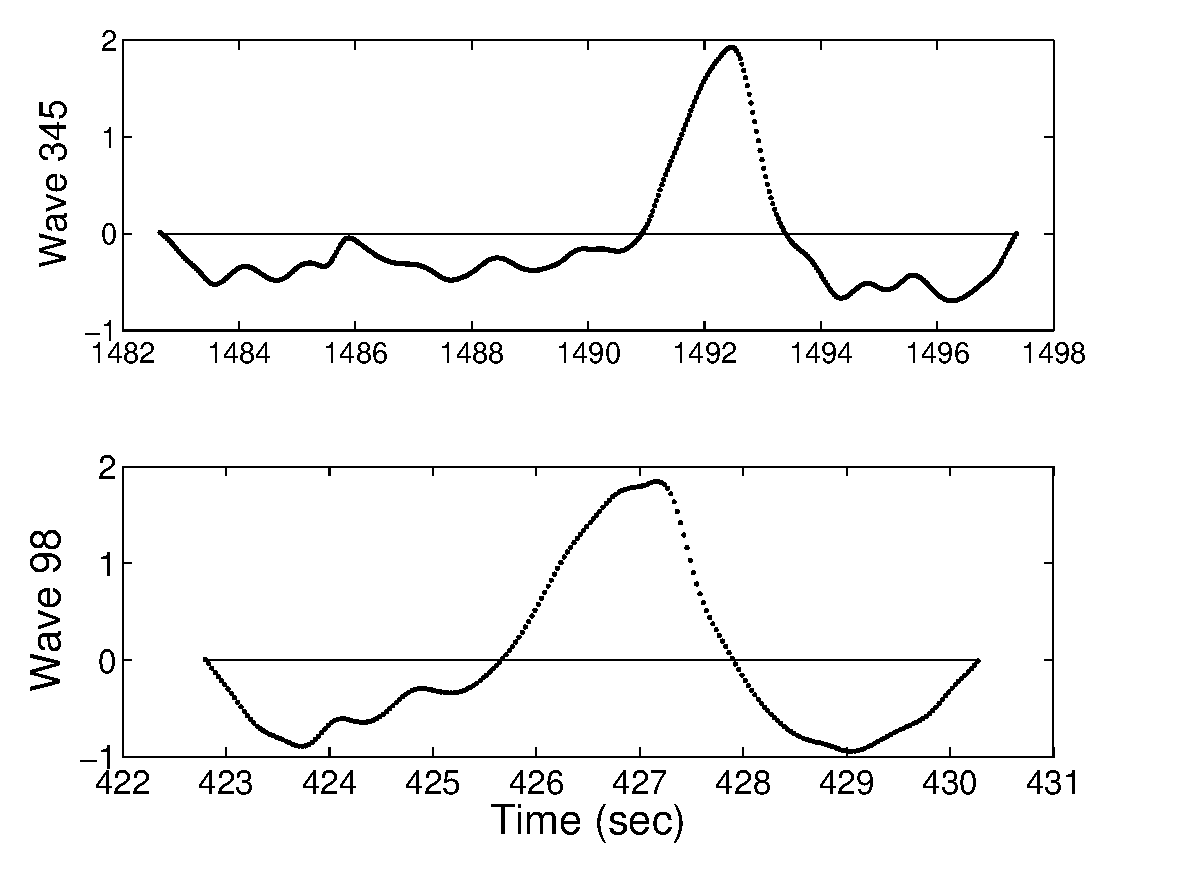
\includegraphics[width=\defwidth]{fig_c_wave}
\end{minipage}}%
\hfill
\subfigure[]{%
\begin{minipage}[b]{0.5\textwidth}%
\centering 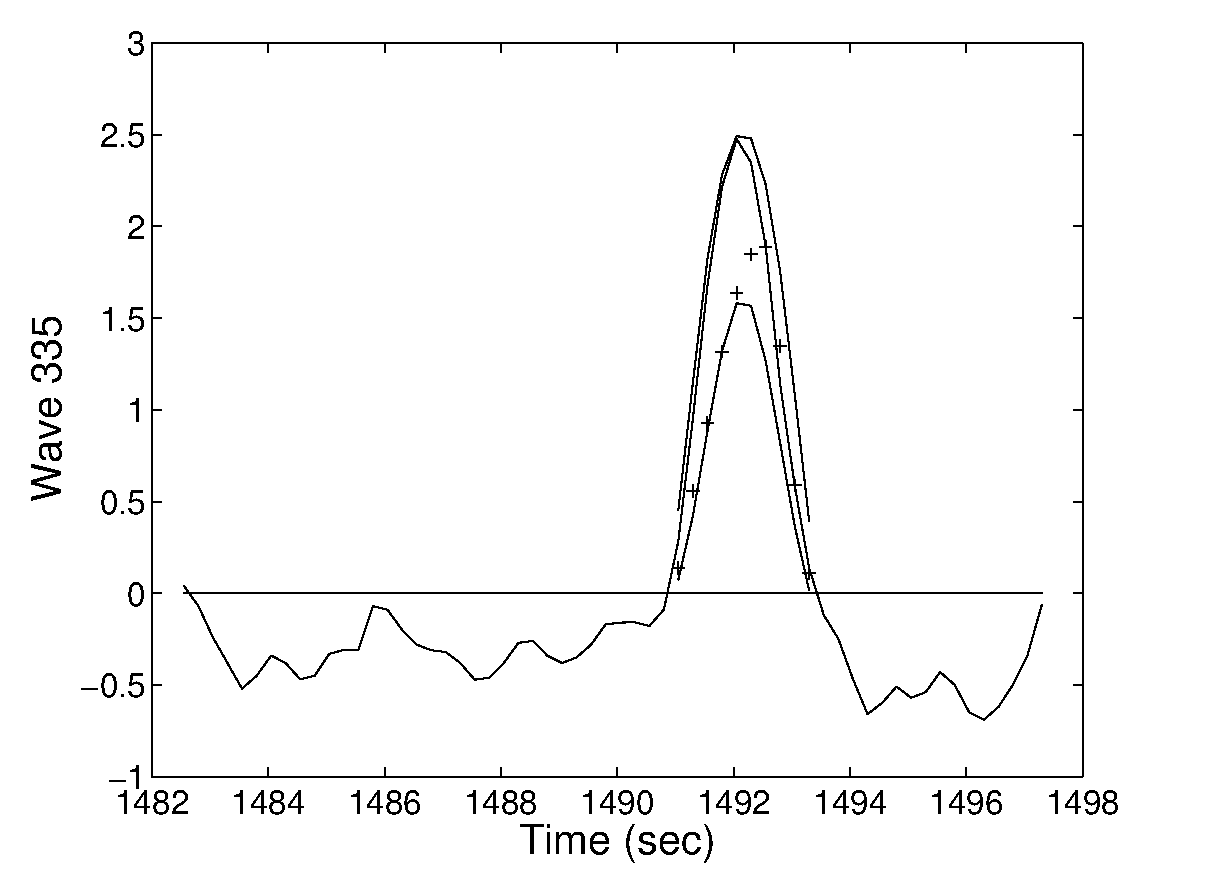
\includegraphics[width=\defwidth]{fig_r_wave}%{Figure33b2017}
\end{minipage}}%
\vspace{-3mm}
  \caption[Reconstructing the highest wave in  {\tt sea.dat}]{
(a): Two waves, the highest and the steepest, observed in {\tt sea.dat}.
(b): Crosses are observations removed from the highest wave.
The reconstructed wave,
using transformed Gaussian model, is given by the middle
solid line. Upper and lower curves give the confidence band defined as the
conditional mean of the process plus minus two conditional standard deviations.
}
\label{fig_c_wave}
\end{figure}

In Figure~\ref{fig_c_wave}(b) the crosses are the removed values from
the wave. The reconstructed wave, plotted by a solid line,
is close to the measured. (Observe that this is a simulated
wave, using the transformed Gaussian model,
and hence each time we execute the command the shape will change.)
The confidence bands gives limits containing 95\% of the simulated
values, pointwise.
From the figure  we can deduce that the highest wave could have been
even higher and that the height is determined by the particularly high
values of the derivatives at the zero crossings which define the wave.
The observed wave looks more asymmetric in time than the reconstructed one.
Such asymmetry is unusual for the transformed Gaussian waves but not
impossible. By executing the following commands we can see that actually the
observed wave is close to the expected in a transformed Gaussian model.
{\small\begin{verbatim}
      plot(xx(inds1,1),xx(inds1,2),'+'), hold on
      mu = tranproc(mu1o,fliplr(grec1));
      plot(y1(inds1,1), mu), hold off
\end{verbatim}}
\noindent
We shall not investigate this question further in this tutorial.
\end{cex}

\subsection{Crest height}
\index[xentr]{wave distributions!estimation of densities!crest height}
We turn now to the kernel estimators of the crest height density.
It is well known that for Gaussian sea the tail of the density is
well approximated by the Rayleigh distribution.
Wand and Jones (1995, Chap. 2.9) show that Gaussian distribution is one
of the easiest distributions to obtain a good Kernel Density Estimate from.
It is more difficult to find good estimates for distributions with
skewness, kurtosis, and multi-modality. Here, one can get help by
transforming data. This can be done choosing different values of input
{\tt L2} into the program {\tt kde}.

\begin{cex}{Ex_sea_statistics}
We shall continue with the analysis of the crest height distribution.
By letting {\tt L2 = 0.6} we see that the normalplot of the transformed data is
approximately linear.
(Note: One should try out several different values for {\tt L2}.
It is also always good practise to try out several different values of
the smoothing parameter; see the help text of {\tt kde} and {\tt kdebin} for
further explanation.)
{\small\begin{verbatim}
      L2 = 0.6;
      plotnorm(Ac.^L2)
      fac = kde(Ac,{'L2',L2},linspace(0.01,3,200));
      pdfplot(fac)
      simpson(fac.x{1},fac.f)
\end{verbatim}}

The integral of the estimated density {\tt fac} is 0.9675 but it should
be one. Therefore, when we use the estimated density to compute different
probabilities concerning the crest height the uncertainty of the computed
probability is at least 0.03. We suspect that this is due to the
estimated density being non-zero for negative values.
In order to check this we compute the
cumulative distribution using the formula,
$$
\pr (Ac\le h)=1-\int_h^{+\infty} f_{Ac}(x)\, \rd x,
$$
where $f_{Ac}(x)$ is the estimated probability density of $Ac$.
For the pdf saved in {\tt fac} the following code gives an estimate of
the cumulative distribution function (cdf) for
crest height and compares it with the empirical distribution
computed from data by means of\index[xcmds]{{\tt plotedf}}
function {\tt edf}\index[xcmds]{{\tt edf}}
or {\tt plotedf}.
{\small\begin{verbatim}
      Fac = flipud(cumtrapz(fac.x{1},flipud(fac.f)));
      Fac = [fac.x{1} 1-Fac];
      Femp = plotedf(Ac,Fac);
      axis([0 2 0 1]), hold off
\end{verbatim}}

Since a kernel density estimator KDE in essence is a smoothed histogram
it is not very well suited for extrapolation of the density to the region
where no data are available, e.g.\ for high crests. In such a case
a parametric model should be used. In \progname{} there is a function
{\tt trraylpdf}\index[xcmds]{{\tt trraylpdf}}
that combines the non-parametric approach of KDE with a Rayleigh density.
Simply, if the Rayleigh variable can be used to described the crests of
Gaussian waves then a transformed Rayleigh variable should be used for
the crests of the transformed Gaussian waves.
The method has several nice properties and will be described more in
Section~\ref{ss:Rayleighappr}. Here we just use it in order to compare with
the non-parametric KDE method.
{\small\begin{verbatim}
      facr = trraylpdf(fac.x{1},'Ac',grec1);
      Facr = cumtrapz(facr.x{1},facr.f); hold on
      plot(facr.x{1},Facr,'.')
      axis([1.25 2.25 0.95 1]), hold off
\end{verbatim}}

Figure \ref{fig_Ac1}(a) shows that our hypothesis that the pdf {\tt fac}
is slightly too low for small crests seems to be correct. Next
from Figure~\ref{fig_Ac1}(b) we can see that also the tail is
reasonably well modelled even if it is lighter than, i.e.\ gives smaller
probabilities of high waves than, the one derived from the transformed
Gaussian model.
\end{cex}

\begin{figure}
\subfigure[]{%
\begin{minipage}[b]{0.5\textwidth}%
\centering 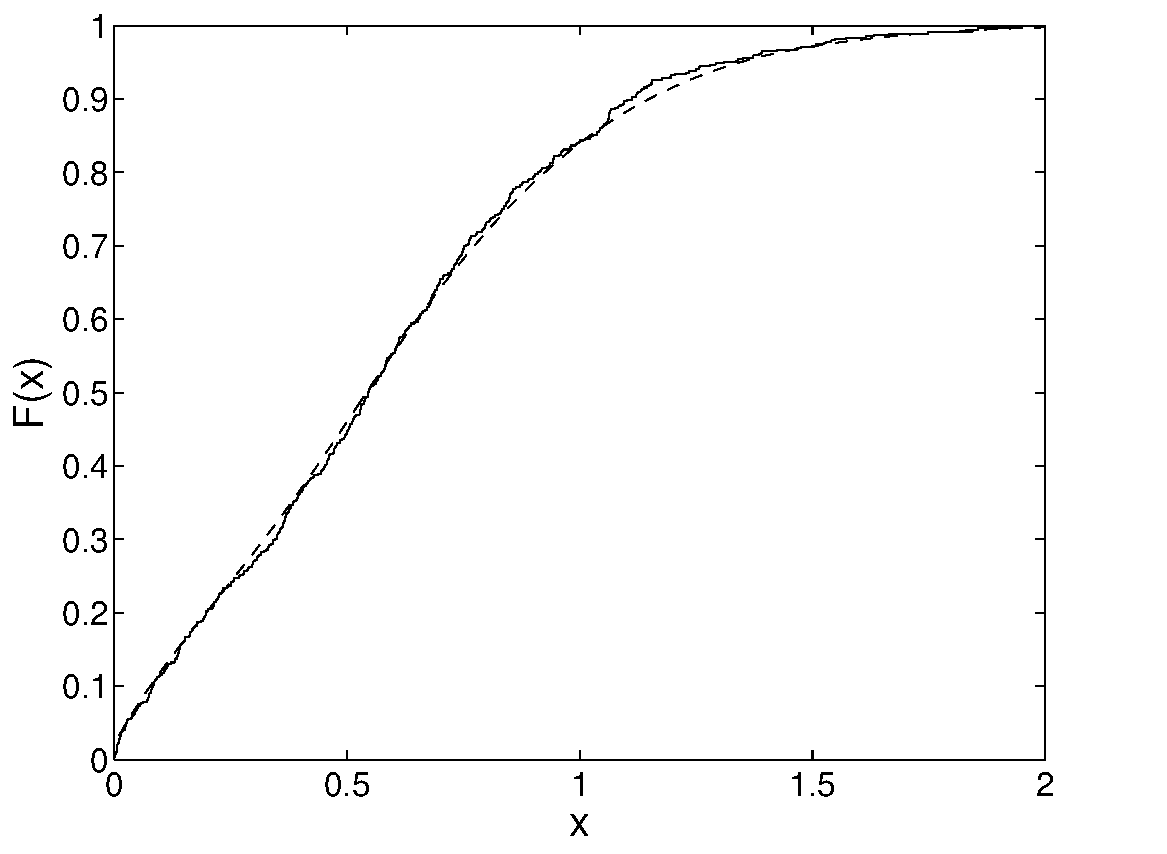
\includegraphics[width=\defwidth]{fig_Ac1}
\end{minipage}}%
\hfill
\subfigure[]{%
\begin{minipage}[b]{0.5\textwidth}%
\centering 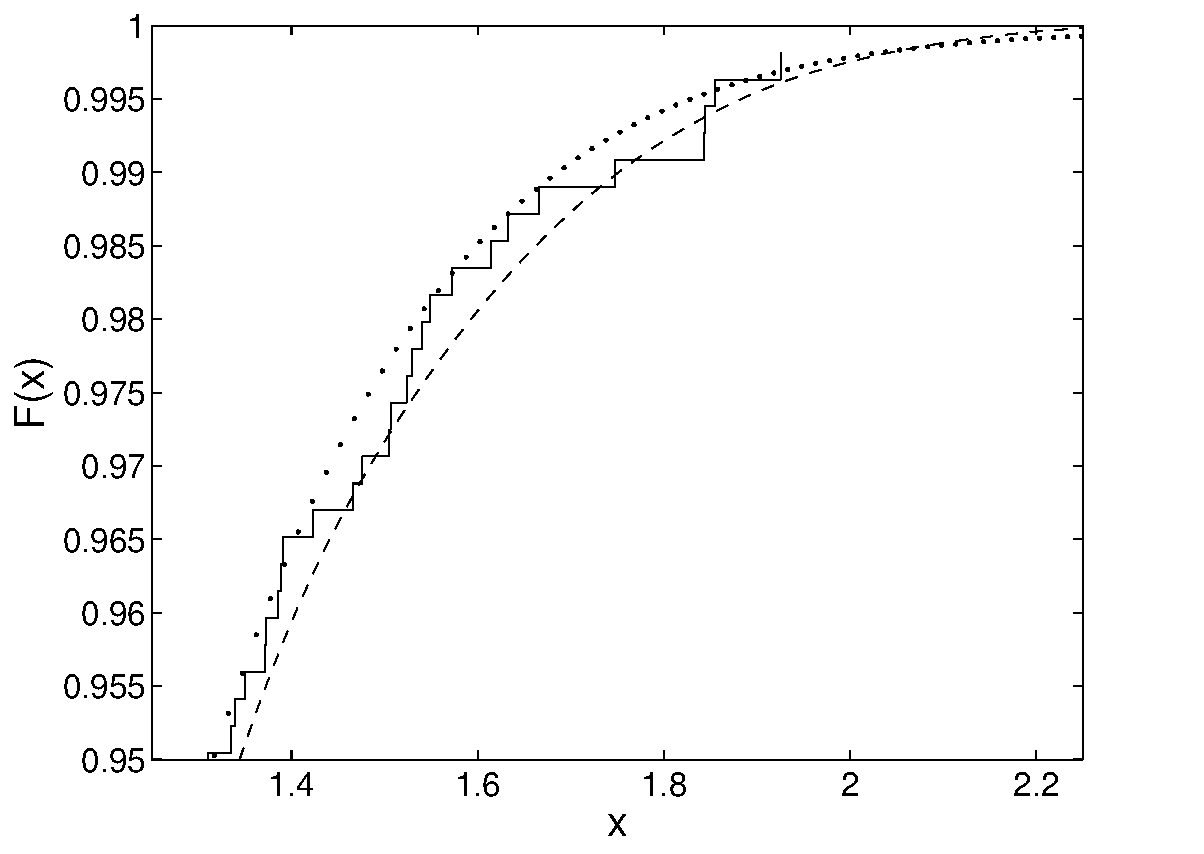
\includegraphics[width=72mm]{fig_Ac2}
\end{minipage}}%
\vspace{-3mm}
  \caption[Comparing different crest height models]{
(a) Comparison of the empirical distribution of the crest height with
the cumulative distribution computed from the KDE estimator.
(b) Zooming in on the tails of distributions in (a) together with
the tail of the transformed Rayleigh approximation (dots) to the crest
height distribution.
}
  \label{fig_Ac1}
\end{figure}

\subsection{Joint crest period and crest height distribution}
\index[xentr]{wave distributions!estimation of densities!
joint crest period and height}
We shall use the kernel density estimator to find a good estimator of
the central part of the joint density of crest period and crest
height. Usually, kernel density estimators give poor estimates
of the tail of the distribution, unless large amounts of data is
available. However, a KDE gives qualitatively good estimates in
regions with sufficient data, i.e.\, in the  main part of the
distribution. This is good for visualization (\verb+pdfplot+) and detecting
modes, symmetries (anti-symmetry) of distributions.

\begin{cex}{Ex_sea_statistics} The following command examines and
  plots the joint distribution of crest period {\tt Tc = Tcf+Tcb}
  and crest height {\tt Ac} in \verb+sea.dat+.
{\small\begin{verbatim}
      kopt2 = kdeoptset('L2',0.5,'inc',256);
      Tc = Tcf+Tcb;
      fTcAc = kdebin([Tc Ac],kopt2);
      fTcAc.labx={'Tc [s]'  'Ac [m]'} % make labels for the plot
      pdfplot(fTcAc), hold on
      plot(Tc,Ac,'k.'), hold off
\end{verbatim}}

\begin{figure}
\centering
   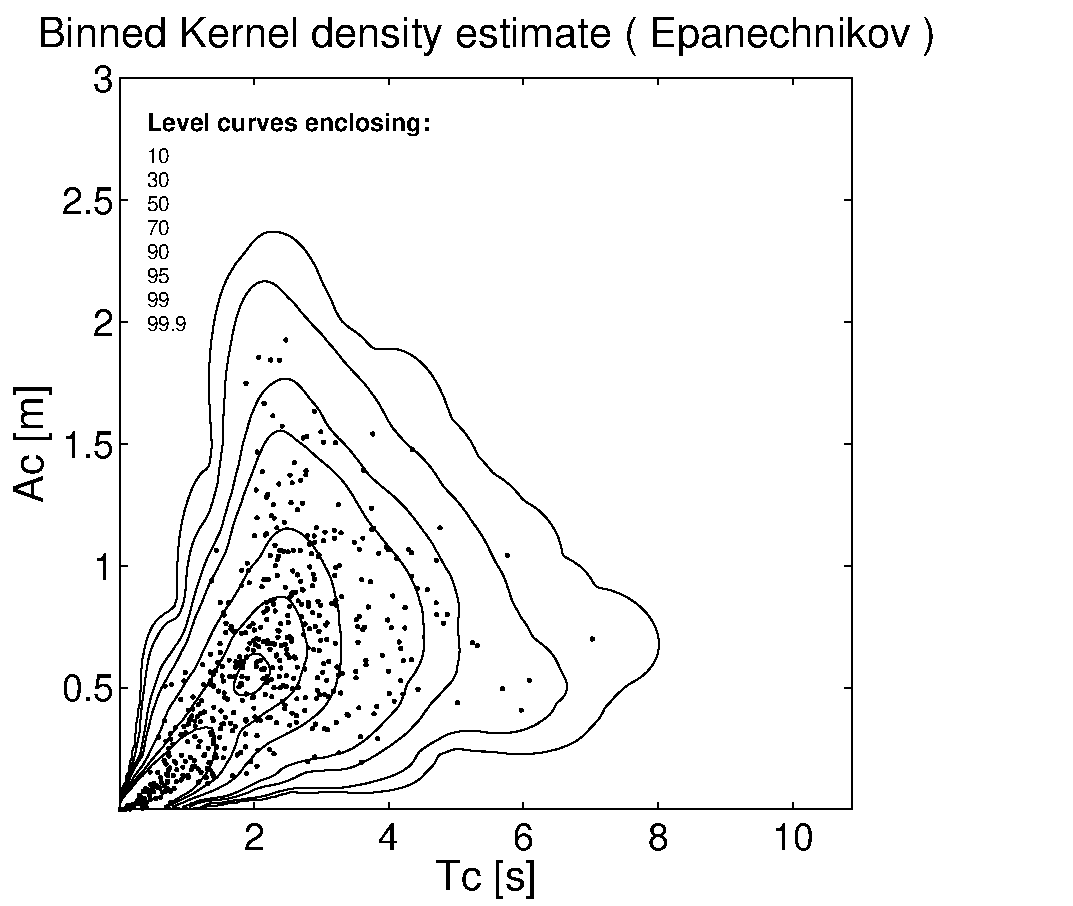
\includegraphics[width=\narrowfigwidth]{fig_TcAc}
\vspace{-3mm}
  \caption[Kernel estimate of the joint density of crest period and
crest height]{
Kernel estimate of joint density of crest period {\tt Tc} and
crest height {\tt Ac} in {\tt sea.dat} compared with the observed data
(dots). The contour lines are drawn in such a way that they contain
specified (estimated) proportions of data.
}
  \label{fig_TcAc}
\end{figure}

In Figure~\ref{fig_TcAc} are plotted 544 pairs of crest period and
height. We can see that the kernel estimate describes the
distribution of data quite well. It is also obvious that it can not be
used to extrapolate outside the observation range. In the following
chapter we shall compute the theoretical joint density of crest period
and height from the transformed Gaussian model and compare with the
KDE estimate.
\end{cex}\index[xentr]{wave characteristics!estimation from data|)}

\section{Explicit results - parametric wave models}
\label{sec:explicitresults_wavemodels}
\index[xentr]{wave models|(}

In this section we shall consider the Gaussian sea with well-defined spectrum. We assume that the
reference level is zero. We will
present some explicit results that are known and
studied in the literature about wave characteristics. Some of them are
exact, others are derived by simplification of the random functions
describing the sea surface.

\subsection{The average wave}
For Gaussian waves the spectrum and the spectral moments contain exact
information about the average behaviour of many wave
characteristics. The \progname{} routines
\verb+spec2char+\index[xcmds]{{\tt spec2char}} and
\verb+spec2bw +\index[xcmds]{{\tt spec2bw}}
compute a long list of wave characteristic parameters.


\begin{rtex}{Ex_wave_parameters}{Simple wave characteristics obtained
    from spectral density}
We start by defining a {\sc Jonswap} spectrum, describing a sea state with
$T_p = 10$ [s], $H_{m_0} = 5$ [m]. Type \verb+spec2mom+ to see what
spectral moments are computed. \index[xcmds]{{\tt spec2mom}}
{\small\begin{verbatim}
     SJ = jonswap([],[5 10]);
     [m mt]= spec2mom(SJ,4,[],0);
\end{verbatim}}

The most basic information about waves is contained
in the spectral moments. The variable {\tt mt} now contains information
about what kind of moments have been computed, in this case spectral
moments up to order four ($m_0, \ldots , m_4$). Next, the irregularity
factor $\alpha$, significant wave height, zero crossing wave period,
and peak period can be computed.
{\small\begin{verbatim}
      spec2bw(SJ)
      [ch Sa2] = spec2char(SJ,[1  3])
\end{verbatim}}

The interesting feature of the  program {\tt spec2char} is that it
also computes an estimate of the variance of the characteristics, given
the length of observations (assuming the Gaussian sea); see
\cite{KrogstadEtal1999Methods}, \cite{Tucker1993recommended}, %,Tu93}
and \cite{Young1999Wind} %,Yo99}
for more detailed
discussion. For example, for the {\sc Jonswap} Gaussian sea,
the standard deviation of significant wave height estimated from 20 minutes
of observations is approximately 0.25~meter.
\end{rtex}

\subsection{Explicit approximations of wave distributions}
\label{sec:explicit_approximations}
\index[xentr]{crest densities|see wave distributions}

\index[xcmds]{{\tt wavemodels}}
\index[xcmds]{{\tt perioddef}}
\index[xcmds]{{\tt ampdef}}
In the module {\tt wavemodels}, we have implemented some of
the approximative models that have been suggested in the literature.
To get an overview of the routines in the module, use the help function on
{\tt wavemodels}.

We will investigate two suggested approximations for the joint pdf of
{\tt (Tc,Ac)}; for the nomenclature, see the routines {\tt perioddef} and
{\tt ampdef} in the module {\tt docs}. Both  functions
need spectral moments as inputs. One should bear in mind that the
models only depend on a few spectral moments and not
on the full wave spectrum.

\subsubsection*{Model by Longuet-Higgins}  %------------
% Parametrization as in Srokosz and Challenor
\index[xentr]{wave models!Longuet-Higgins}
\index[xentr]{wave distributions!approximative densities!
Longuet-Higgins}
Longuet-Higgins,
\cite{Longuet-Higgins1975Joint,Longuet-Higgins1983Joint}, derived his
approximative distribution by considering the joint
distribution of the envelope amplitude and the time derivative of the
envelope phase. The model is valid for narrow-band processes.
It seams to give relatively accurate results for big waves, e.g.\
for waves with significant amplitudes.

The Longuet-Higgins density depends, besides
the significant wave height $H_s$ and peak period $T_p$, on
the spectral width parameter
$ \nu = \frac{m_0m_2}{m_1^2}-1$,
which can be calculated by the command {\tt spec2bw(S,'eps2')},
(for a narrow-band process, $\nu \approx 0$). The explicit density is
given by
\[
f^{\mbox{\scriptsize{LH}}}_{T_c,A_c}(t,x)=c_{\mbox{\scriptsize{LH}}}\,
\left(\frac{x}{t}\right)^2 \exp\left\{
    -\frac{x^2}{8}\big[1+\nu^{-2}(1-t^{-1})^2\big] \right\} ,
\]
where
\[
c_{\mbox{\scriptsize{LH}}}=\frac{1}{8}(2\pi)^{-1/2}\nu^{-1}[
  1+(1+\nu^2)^{-1/2}]^{-1}.
\]
The density is calculated by the
function \verb+lh83pdf+. \index[xcmds]{{\tt lh83pdf}}

\begin{cex}{Ex_wave_parameters} For the Longuet-Higgins approximation of the 
$T_c,A_c$ distribution for {\sc Jonswap} waves we use the spectral moments just calculated.
{\small\begin{verbatim}
      t = linspace(0,15,100);
      h = linspace(0,6,100);
      flh = lh83pdf(t,h,[m(1),m(2),m(3)]);
\end{verbatim}}

%%%%%%%%%%%%%% Figure L-H %%%%%%%%%%%%%%%%%%%%%%%

\begin{figure}
\subfigure[]{%
\begin{minipage}[b]{0.5\textwidth}%
\centering 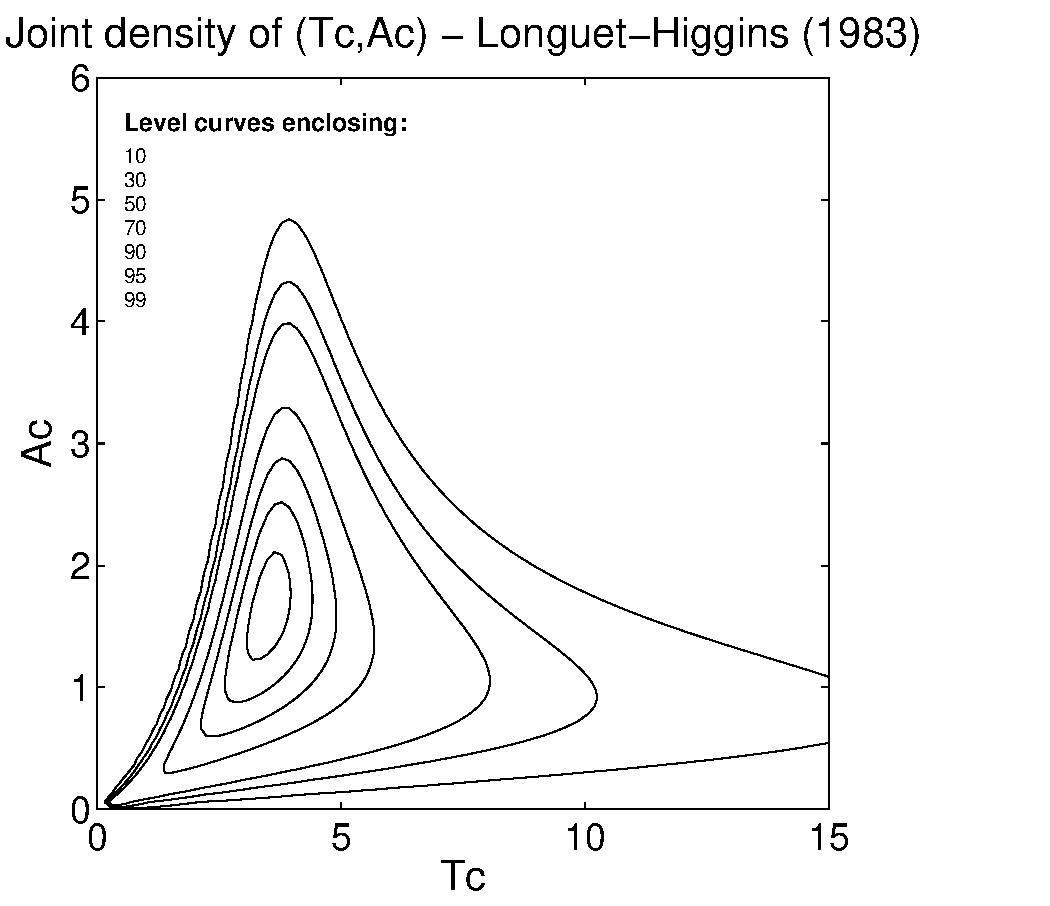
\includegraphics[width=\defwidth]{lhdens}
\end{minipage}}%
\hfill
\subfigure[]{%
\begin{minipage}[b]{0.5\textwidth}%
\centering 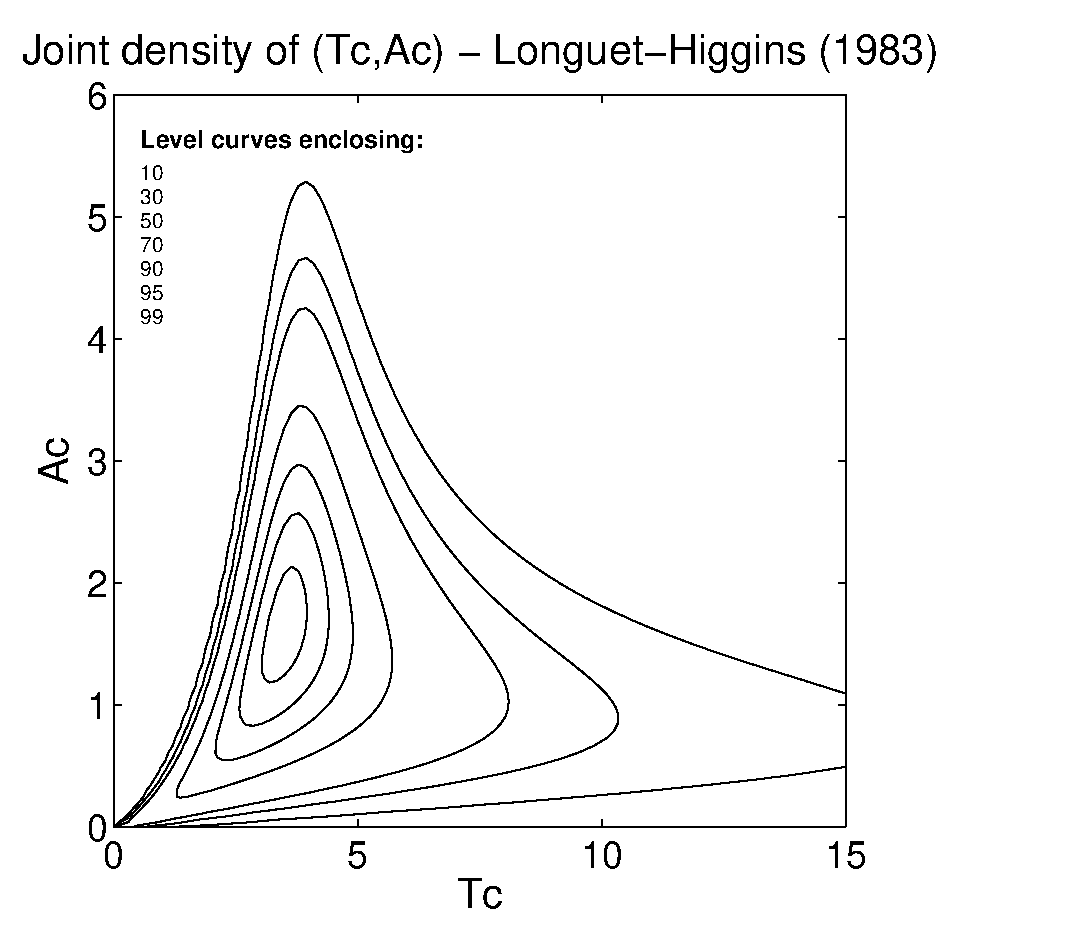
\includegraphics[width=\defwidth]{lhdens1}
\end{minipage}}
\vspace{-3mm}
  \caption[Longuet-Higgins model for joint pdf of crest period and height]{%
Longuet-Higgins model for joint pdf of crest period $T_c$
and crest height $A_c$. Spectrum: JONSWAP with $T_p=10$~[s], $H_{m_0}=5$~[m].
(a) linear Gaussian sea, (b) transformed Gaussian sea.
}
\label{fig:lhdens}
\end{figure}

In \progname{} we have modified the Longuet-Higgins
density to be applicable also for
transformed Gaussian models. Following the examples from the previous chapter
we compute the transformation proposed by Winterstein and combine it with
the Longuet-Higgins model.
{\small\begin{verbatim}
      [sk, ku] = spec2skew(SJ);
      sa = sqrt(m(1));
      gh = hermitetr([],[sa sk ku 0]);
      flhg = lh83pdf(t,h,[m(1),m(2),m(3)],gh);
\end{verbatim}} \index[xcmds]{{\tt spec2skew}}\index[xcmds]{{\tt hermitetr}}

In Figure~\ref{fig:lhdens} the densities {\tt flh} and {\tt flhg} are
compared. The contour lines are drawn in such a way that they contain
predefined proportions of the total probability mass inside the
contours. We can see that including some nonlinear effects
gives somewhat higher waves for the {\sc Jonswap} spectrum.
\end{cex}

 %%%%%%%%%%%%%%%%%%%%%%%%%%%%%%%%%%%%%%%%%%%%
\subsubsection*{Model by Cavani\'e et al.} %------------
% Parametrization as in Srokosz and Challenor!
\index[xentr]{wave models!Cavani\'e et al.}
\index[xentr]{wave distributions!approximative densities!
Cavani\'e et al.}
Another explicit density for the crest height was proposed
by Cavani{\' e} et al., \cite{CavanieEtal1976Statistical}.
Here any positive local maximum is considered
as a crest of a wave, and then the second derivative (curvature) at the
local maximum defines the wave period as if the entire wave was a cosine function
with the same height and the same crest curvature.

The model uses the parameter $\nu$  and a higher order bandwidth
parameter\footnote{The value of $\epsilon$ may be
  calculated by {\tt spec2bw(S,'eps4')}}
$\epsilon$, defined by
\begin{align*}
\epsilon &= \sqrt{1-\frac{m_2^2}{m_0m_4}};
\end{align*}
where, for a narrow-band process, $\epsilon \approx 0$. The
  Cavani{\'e} distribution is given by
\begin{align*}
f^{\mbox{\scriptsize{CA}}}_{T_c,A_c}(t,x) &=
c_{\mbox{\scriptsize{CA}}}
\frac{x^2}{t^5}\exp \left \{-\frac{x^2}{8\varepsilon^2 t^4}\left[
\left( t^2-\left(\frac{1-\varepsilon^2}{1+\nu^2}\right)\right)^2+
\beta^2\left(\frac{1-\varepsilon^2}{1+\nu^2}\right)\right]\right\},
\intertext{where}
c_{\mbox{\scriptsize{CA}}} &=
  \frac{1}{4}(1-\epsilon^2)(2\pi)^{-1/2}{\epsilon}^{-1}
             {\alpha_2}^{-1}(1+\nu^2)^{-2}, \\
  {\alpha}_2 &= \frac{1}{2}[1+(1-{\epsilon}^2)^{1/2}], \\
  \beta &= {\epsilon}^2/(1-{\epsilon}^2) .
  \end{align*}
The density is computed by
{\small\begin{verbatim}
      t = linspace(0,10,100);
      h = linspace(0,7,100);
      fcav = cav76pdf(t,h,[m(1) m(2) m(3) m(5)],[]);
\end{verbatim}}\index[xcmds]{{\tt cav76pdf}}

\noindent
and a contour plot of the pdf is obtained by {\tt pdfplot(fcav)};
see~Figure~\ref{fig:cavdens}.

%%%%%%%%%%%%%%%%%%%%%%%%%%%%%% Figure Cavanie %%%%%%%%%%%
\begin{figure}
\subfigure[]{%
\begin{minipage}[b]{0.45\textwidth}%
\centering
%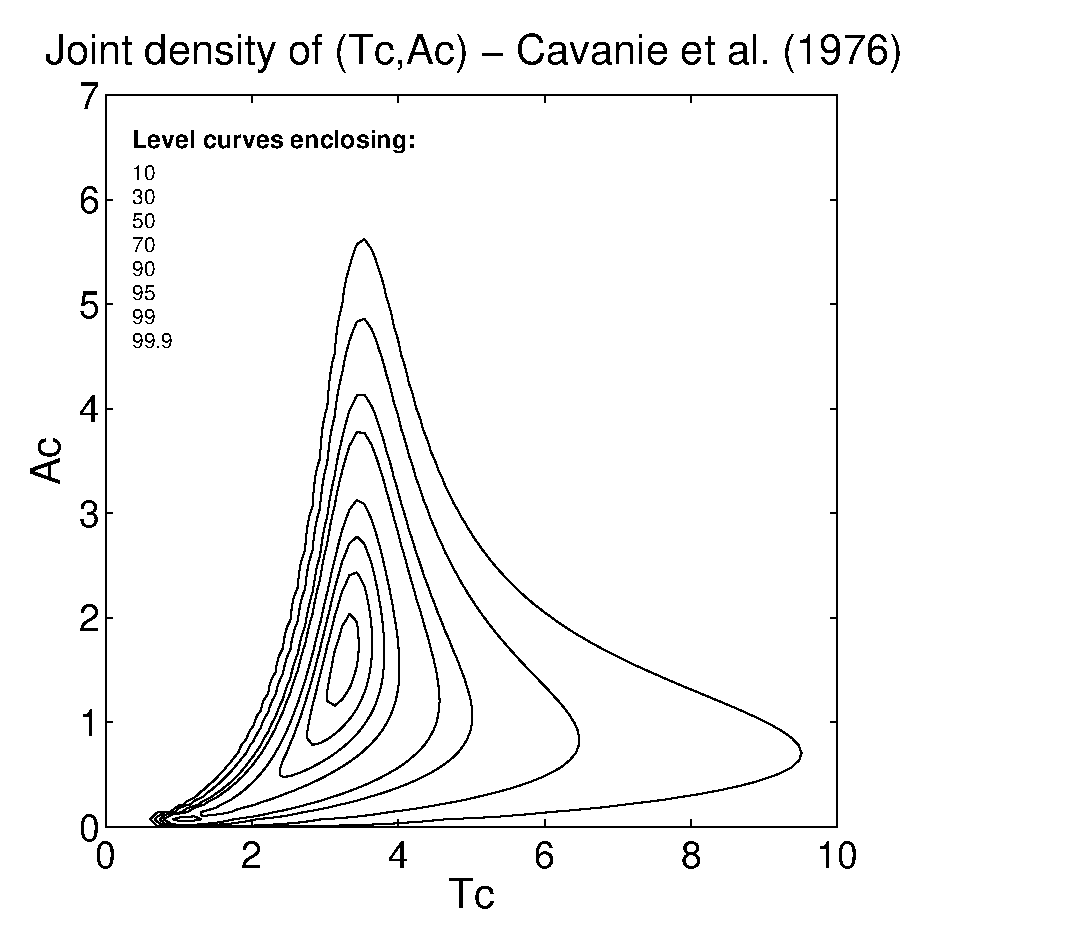
\includegraphics[height=\defheight]{cavdens}
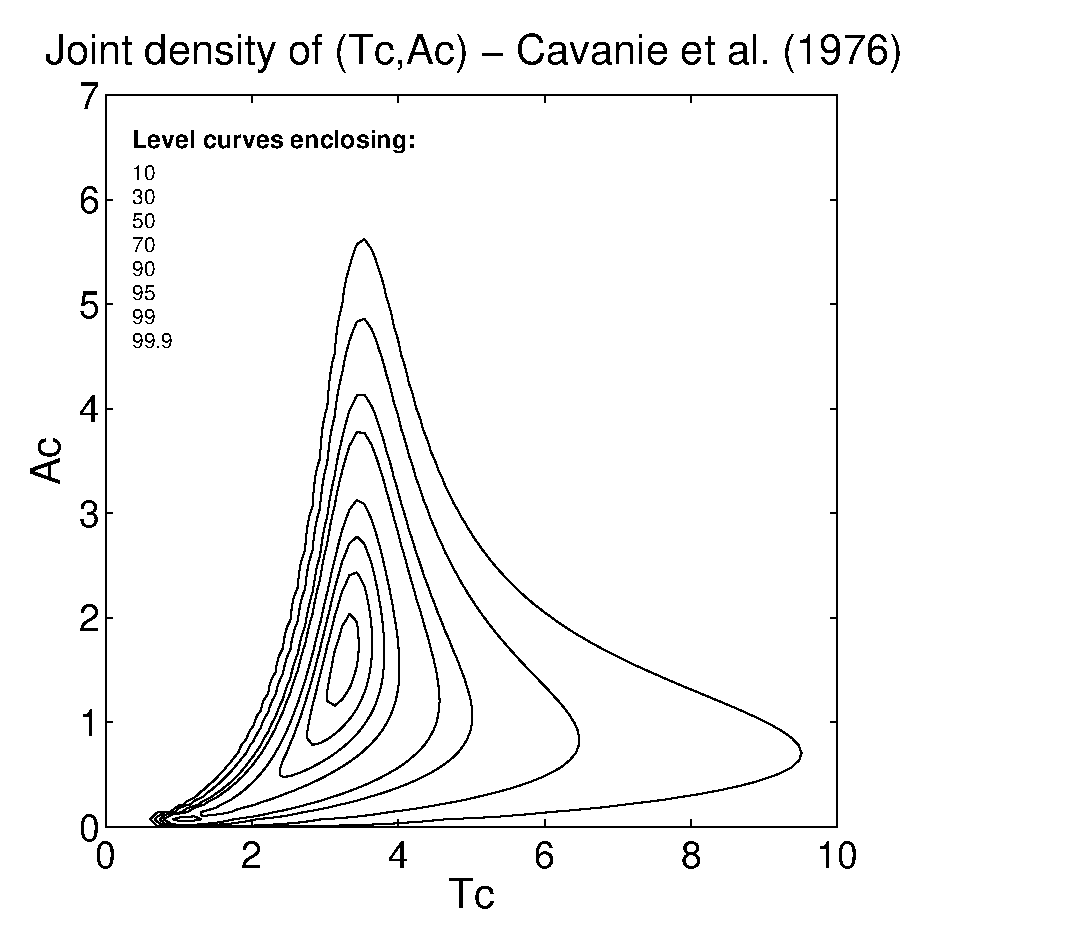
\includegraphics[height=58mm]{cavdens}
\end{minipage}}%
\hspace{0mm}
%\hfill
\subfigure[]{%
\begin{minipage}[b]{0.54\textwidth}%
\centering
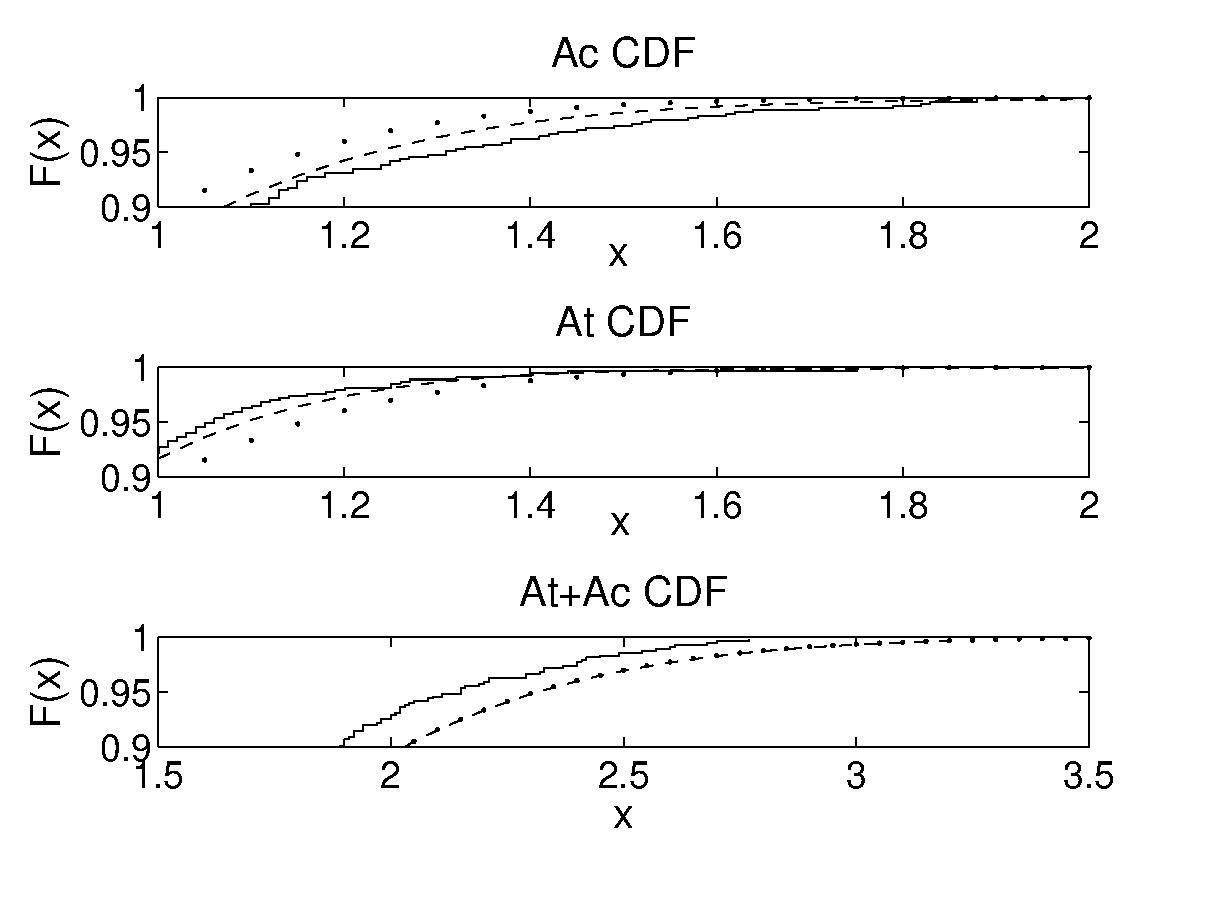
\includegraphics[height=58mm]{figAcAt_h}
\end{minipage}}
\vspace{-3mm}
  \caption[Joint density of crest period and
crest height by Cavani\'e et al]{
(a) Contour lines of the joint density of crest period and
crest height proposed by Cavani\'e et al, for Gaussian sea with
{\sc Jonswap} spectrum ($T_p=10$ [s], $H_{m_0}=5$ [m]). (b) The tail of the
empirical distribution of crest height (top), trough depth (middle) and
amplitude (bottom) compared with Rayleigh approximation (dots) and
transformed Rayleigh model with Hermite transformation.
}
  \label{fig:cavdens}
\end{figure}
%%%%%%%%%%%%%%%%%%%%%%%%%%%%%%%%%%%%%%%%%%%%%%%%%%%%%

\subsection{Rayleigh approximation for wave crest height}\label{ss:Rayleighappr}
\index[xentr]{wave distributions!approximative densities!
Rayleigh approximation}\label{ss:Rayleighapproximation}
There are several densities proposed in the literature to approximate
the height of a wave crest or its amplitude. Some of them are programmed
in \progname{}; execute {\tt help wavemodels} for a list.
For Gaussian sea the most simple and most
frequently used model is the Rayleigh
density. The standardized Rayleigh variable $R$ has probability density 
$f(r)=r\exp(-r^2/2)$, $x > 0$. It is well known that for Gaussian sea
the Rayleigh approximation works very well for high waves,
and actually it is a conservative approximation since we have
$$
\pr (A_c > h) \leq \pr (R> 4 h/H_s) = e^{-8h^2/H_s^2},
$$
see \cite{RyclikAndLeadbettter1997Analysis}.
In that paper it is also shown that for any sea wave model with
crossing intensity $\mu(u)$, one has $\pr (A_c>h) \leq \mu(u)/\mu(0)$.
The approximation becomes more accurate as the level $h$
increases.

The crossing intensity $\mu(u)$ is given by
Rice's formula, Rice (1944),\index[xentr]{Rice's formula}
\index[xentr]{crossing intensity!Rice's formula}
and it can be computed when the joint density of sea level $X(t)$ and its
derivative $X'(t)$ is known, see Section~\ref{subsec:crossing_intensity},
$$
\mu(u) = \int_0^{\infty} zf_{X(t), X'(t)}(u,z)\,\rd z.
$$
For a Gaussian sea it can be computed explicitly,
$$
\mu(u) = \frac{1}{T_z} e^{-8u^2/H_s^2}.
$$
For non-linear wave models with random Stokes waves the crossing
intensity has to be computed using numerical integration; see the
work  by Machado and Rychlik,
\cite{MachadoAndRychlik2003Wave}.

Knowing the crossing intensity $\mu(u)$ one can compute the
transformation $g$, by using the routine
{\tt lc2tr}\index[xcmds]{{\tt lc2tr}}, such that  the transformed
Gaussian model has crossing intensity equal to $\mu(u)$. Consequently,
we have that \index[xcmds]{{\tt ls2tr}}
$
\pr (A_c>h) \leq \pr (R> g(h)) = 1- \pr (G(R)\leq h).$
The function {\tt trraylpdf} computes the pdf of $G(R)$. (Obviously
the function works for any transformation $g$.)
\index[xcmds]{{\tt trraylpdf}}

In previous examples we used the estimated crossing intensity to
compute the transformation and then approximated the crest height
density using the transformed Rayleigh variable.
The accuracy of the approximation for the high crests in
the data set {\tt xx = sea.dat} was checked, see Figure~\ref{fig_Ac1}(b).
A more extensive study of the applicability of this approximation
is done in \cite{RyclikAndLeadbettter1997Analysis}.


\begin{rtex}{rayleighapproximation}{Rayleigh approximation of crest
height from spectral density}
In this example we shall use a transformed Rayleigh approximation for
crest height derived from a sea spectrum. In order to check the
accuracy of the approximations we shall use the estimated spectrum
from the record {\tt sea.dat}.
{\small\begin{verbatim}
      xx = load('sea.dat');
      x = xx;
      x(:,2) = detrend(x(:,2));
      SS = dat2spec2(x);
      [sk, ku, me, si] = spec2skew(SS);
      gh = hermitetr([],[si sk ku me]);
      Hs = 4*si;
      r = (0:0.05:1.1*Hs)';
      fac_h = trraylpdf(r,'Ac',gh);
      fat_h = trraylpdf(r,'At',gh);
      h = (0:0.05:1.7*Hs)';
      facat_h = trraylpdf(h,'AcAt',gh);
      pdfplot(fac_h), hold on
      pdfplot(fat_h), hold off
\end{verbatim}}

Next, we shall compare the derived approximation with the observed
crest heights in {\tt x}. As before, we could use the function {\tt dat2steep}
to find the crests. Here, for illustration only,  we shall use
{\tt dat2tc}\index[xcmds]{{\tt dat2tc}}
to find the crest heights {\tt Ac} and trough depth {\tt At}.
{\small\begin{verbatim}
      TC = dat2tc(xx, me);
      tc = tp2mm(TC);
      Ac = tc(:,2); At = -tc(:,1);
      AcAt = Ac+At;
\end{verbatim}}

Finally, the following commands will give the cumulative distributions
for the computed densities.
{\small\begin{verbatim}
      Fac_h = [fac_h.x{1} cumtrapz(fac_h.x{1},fac_h.f)];
      subplot(3,1,1)
      Fac = plotedf(Ac,Fac_h); hold on
      plot(r,1-exp(-8*r.^2/Hs^2),'.')
      axis([1. 2. 0.9 1])
      Fat_h = [fat_h.x{1} cumtrapz(fat_h.x{1},fat_h.f)];
      subplot(3,1,2)
      Fat = plotedf(At,Fat_h); hold on
      plot(r,1-exp(-8*r.^2/Hs^2),'.')
      axis([1. 2. 0.9 1])
      Facat_h = [facat_h.x{1} cumtrapz(facat_h.x{1},facat_h.f)];
      subplot(3,1,3)
      Facat = plotedf(AcAt,Facat_h); hold on
      r2 = (0:05:2.1*Hs)';
      plot(r2,1-exp(-2*r2.^2/Hs^2),'.')
      axis([1.5 3.5 0.9 1]), hold off
\end{verbatim}}

In Figure~\ref{fig:cavdens}(b) we can see some differences between the
observed crest and trough distributions and those obtained from the
transformation {\tt gh}.  However, it still gives a much better
approximation than the standard Rayleigh approximation (dots).
As it was shown before, using the transformation computed from the
crossing intensity, the transformed Rayleigh approach is giving
a perfect fit. Finally, one can see that the Rayleigh and transformed
Rayleigh variables give too conservative approximations to
the distribution of wave amplitude.
\end{rtex}\index[xentr]{wave models|)}

%\begin{comment}
\newpage
\section{\progname{} wave characteristics}\label{sec:WAFOcharacteristics}

\subsection{spec2char}\label{ss:spectralcharacteristics}
\index[xentr]{wave characteristics!computation from spectrum}
{\small\begin{verbatim}
help spec2char

 SPEC2CHAR Evaluates spectral characteristics and their variance

 CALL: [ch r chtext] = spec2char(S,fact,T)

       ch = vector of spectral characteristics
       r  = vector of the corresponding variances given T
   chtext = a cellvector of strings describing the elements of ch
       S  = spectral struct with angular frequency
     fact = vector with factor integers, see below.
            (default [1])
       T  = recording time (sec) (default 1200 sec = 20 min)

 If input spectrum is of wave number type, output are factors
 for corresponding 'k1D', else output are factors for 'freq'.
 Input vector 'factors' correspondence:
    1 Hm0   = 4*sqrt(m0)           Significant wave height
    2 Tm01  = 2*pi*m0/m1           Mean wave period
    3 Tm02  = 2*pi*sqrt(m0/m2)     Mean zero-crossing period
    4 Tm24  = 2*pi*sqrt(m2/m4)     Mean period between maxima
    5 Tm_10 = 2*pi*m_1/m0          Energy period
    6 Tp    = 2*pi/{w | max(S(w))} Peak period
    7 Ss    = 2*pi*Hm0/(g*Tm02^2)  Significant wave steepness
    8 Sp    = 2*pi*Hm0/(g*Tp^2)    Average wave steepness
    9 Ka    = abs(int S(w) exp(i*w*Tm02) dw) / m0
                                   Groupiness parameter
   10 Rs    = se help spec2char    Quality control parameter
   11 Tp    = 2*pi*int S(w)^4 dw   Peak Period
              ------------------   (more robust estimate)
              int w*S(w)^4 dw

   12 alpha = m2/sqrt(m0*m4)       Irregularity factor
   13 eps2  = sqrt(m0*m2/m1^2-1)   Narrowness factor
   14 eps4  = sqrt(1-m2^2/(m0*m4)) = sqrt(1-alpha^2)  Broadness factor
   15 Qp    = (2/m0^2)int_0^inf w*S(w)^2 dw           Peakedness factor

 Order of output is same as order in 'factors'
 The variances are computed with a Taylor expansion technique
 and is currently only available for factors 1,2 and 3.
\end{verbatim}}\index[xcmds]{{\tt spec2char}}

\newpage
\subsection{spec2bw}
{\small\begin{verbatim}
help spec2bw

 SPEC2BW Evaluates some spectral bandwidth and irregularity factors

  CALL:  bw = spec2bw(S,factors)

         bw = vector of factors
         S  = spectrum struct
    factors = vector with integers, see below. (default [1])

  If input spectrum is of wave-number type, output are factors for
  corresponding 'k1D', else output are factors for 'freq'.
  Input vector 'factors' correspondence:
     1 alpha=m2/sqrt(m0*m4)                        (irregularity factor)
     2 eps2 = sqrt(m0*m2/m1^2-1)                   (narrowness factor)
     3 eps4 = sqrt(1-m2^2/(m0*m4))=sqrt(1-alpha^2) (broadness factor)
     4 Qp=(2/m0^2)int_0^inf f*S(f)^2 df            (peakedness factor)
  Order of output is the same as order in 'factors'

  Example:
    S=demospec;
    bw=spec2bw(S,[1 2 3 4]);
\end{verbatim}} \index[xcmds]{{\tt spec2bw}}

\newpage
\subsection{wavedef}\index[xentr]{wave characteristics!definitions}
{\small\begin{verbatim}
help wavedef

  WAVEDEF wave definitions and nomenclature

  Definition of trough and crest:
 ~~~~~~~~~~~~~~~~~~~~~~~~~~~~~~~~
  A trough (t) is defined as the global minimum between a
  level v down-crossing (d) and the next up-crossing (u)
  and a crest (c) is defined as the global maximum between
  a level v up-crossing and the following down-crossing.

  Definition of down- and up-crossing waves:
 ~~~~~~~~~~~~~~~~~~~~~~~~~~~~~~~~~~~~~~~~~~~~~
  A level v-down-crossing wave (dw) is a wave from a
  down-crossing to the following down-crossing.
  Similarly a level v-up-crossing wave (uw) is a wave from
  an up-crossing to the next up-crossing.

  Definition of trough and crest waves:
 ~~~~~~~~~~~~~~~~~~~~~~~~~~~~~~~~~~~~~~
  A trough to trough wave (tw) is a wave from a trough (t)
  to the following trough.
  The crest to crest wave (cw) is defined similarly.

  Definition of min2min and Max2Max wave:
 ~~~~~~~~~~~~~~~~~~~~~~~~~~~~~~~~~~~~~~~~~
  A min2min wave (mw) is defined starting from a minimum (m)
  and ending in the following minimum.
  A Max2Max wave (Mw) is a wave from a maximum (M) to
  the next maximum (all waves optionally rainflow filtered).

            <----- Direction of wave propagation
    <------Mw-----> <----mw---->
    M             : :  c       :
   / \            M : / \_     :     c_            c
  F   \          / \m/    \    :    /: \          /:\   level v
 ------d--------u----------d-------u----d--------u---d--------
        \      /:           \  :  /: :  :\_    _/  : :\_   L
         \_   / :            \_t_/ : :  :  \t_/    : :  \m/
           \t/  <-------uw---------> :  <-----dw----->
            :                  :     :             :
            <--------tw-------->     <------cw----->
  (F= first value and L=last value).
 See also: tpdef, crossdef, dat2tc, dat2wa, dat2crossind
\end{verbatim}
}\index[xcmds]{{\tt wavedef}}

\newpage
\subsection{perioddef}
{\small\begin{verbatim}
help perioddef

  PERIODDEF wave periods (lengths) definitions and
  nomenclature

  Definition of wave periods (lengths):
 ---------------------------------------

            <----- Direction of wave propagation

                <-------Tu-------->
                :                 :
                <---Tc----->      :
                :          :      : <------Tcc---->
    M           :      c   :      : :             :
   / \          : M   / \_ :      : c_            c
  F   \         :/ \m/    \:      :/  \          / \   level v
 ------d--------u----------d------u----d--------u---d--------
        \      /            \    /     :\_    _/:   :\_   L
         \_   /              \t_/      :  \t_/  :   :  \m/
           \t/                :        :        :   :
            :<-------Ttt----->:        <---Tt--->   :
                                       :<----Td---->:
   Tu   = Wave up-crossing period
   Td   = Wave down-crossing period
   Tc   = Crest period, i.e., period between up-crossing and
          the next down-crossing
   Tt   = Trough period, i.e., period between down-crossing and
          the next up-crossing
   Ttt  = Trough2trough period
   Tcc  = Crest2crest period
\end{verbatim}
}\index[xcmds]{{\tt perioddef}}

\newpage
{\small\begin{verbatim}
            <----- Direction of wave propagation

                 <--Tcf->                           Tuc
                 :      :               <-Tcb->     <->
    M            :      c               :     :     : :
   / \           : M   / \_             c_    :     : c
  F   \          :/ \m/    \           /  \___:     :/ \ level v
 ------d---------u----------d---------u-------d-----u---d-------
       :\_      /            \     __/:        \   /     \_   L
       :  \_   /              \_t_/   :         \t/        \m/
       :    \t/                 :     :
       :     :                  :     :
       <-Ttf->                  <-Ttb->

   Tcf  = Crest front period, i.e., period between up-crossing
          and crest
   Tcb  = Crest back period, i.e., period between crest and
          down-crossing
   Ttf  = Trough front period, i.e., period between
          down-crossing and trough
   Ttb  = Trough back period, i.e., period between trough and
          up-crossing

  Also note that Tcf and Ttf can also be abbreviated by their
  crossing marker, e.g. Tuc (u2c) and Tdt (d2t), respectively.
  Similar rules apply to all the other wave periods and wave
  lengths. (The nomenclature for wave length is similar, just
  substitute T and period with L and length, respectively)

              <----- Direction of wave propagation
                       <--TMm-->
            <-TmM->    :       :
    M       :     :    M       :
   / \      :     M   /:\_     :     M_            M
  F   \     :    / \m/ :  \    :    /: \          / \
       \    :   /      :   \   :   / :  \        /   \
        \   :  /       :    \  :  /  :   \_    _/     \_   L
         \_ : /        :     \_m_/   :     \m_/         \m/
           \m/         :             :      :            :
                       <-----TMM----->      <----Tmm----->

   TmM = Period between minimum and the following Maximum
   TMm = Period between Maximum and the following minimum
   TMM = Period between Maximum and the following Maximum
   Tmm = Period between minimum and the following minimum
See also: wavedef, ampdef, crossdef, tpdef
\end{verbatim}
  }

%\newpage
\subsection{ampdef}
{\small\begin{verbatim}
help ampdef

  AMPDEF wave heights and amplitude definitions and
  nomenclature

  Definition of wave amplitude and wave heights:
 ~~~~~~~~~~~~~~~~~~~~~~~~~~~~~~~~~~~~~~~~~~~~~~~

             <----- Direction of wave propagation

            ...............c_..........
            |             /| \         |
        Hd  |           _/ |  \        |  Hu
    M       |          /   |   \       |
   / \      |     M   / Ac |    \_     |     c_
  F   \     |    / \m/     |      \    |    /  \  level v
 ------d----|---u------------------d---|---u----d------
        \   |  /|                   \  |  /      \L
         \_ | / | At                 \_|_/
           \|/..|                      t
            t

   Ac   = crest amplitude
   At   = trough amplitude
   Hd   = wave height as defined for down-crossing waves
   Hu   = wave height as defined for up-crossing waves

  See also: wavedef, ampdef, crossdef, tpdef
\end{verbatim}
    }\index[xcmds]{{\tt ampdef}}

  \newpage
  \subsection{crossdef}\index[xentr]{level crossing}
\index[xentr]{upcrossing!definition}
  \index[xentr]{downcrossing!definition}
  {\small\begin{verbatim}
help crossdef

  CROSSDEF level v crossing definitions and nomenclature

  Definition of level v crossing:
 ~~~~~~~~~~~~~~~~~~~~~~~~~~~~~~~~
  Let the letters 'm', 'M', 'F', 'L','d' and 'u' in the
  figure below denote local minimum, maximum, first value, last
  value, down- and up-crossing, respectively. The remaining
  sampled values are indicated with a '.'. Values that are
  identical with v, but do not cross the level is indicated
  with the letter 'o'.

  We have a level up-crossing at index, k, if

           x(k) <  v and v < x(k+1)
  or if
           x(k) == v and v < x(k+1) and x(r) < v for some
                     di < r <= k-1

  where di is  the index to the previous down-crossing.
  Similarly there is a level down-crossing at index, k, if

           x(k) >  v and v > x(k+1)
   or if
           x(k) == v and v > x(k+1) and x(r) > v  for some
                     ui < r <= k-1

  where ui is  the index to the previous up-crossing.

  The first (F) value is a up-crossing if x(1) = v and x(2) > v.
  Similarly, it is a down-crossing if     x(1) = v and x(2) < v.

       M
     .   .                  M                   M
   .      . .             .                   .   .
 F            d               .             .       L   level v
  ----------------------u-------d-------o---------------------
                .     .           .   .   u
                  .                 m
                   m

  See also: perioddef, wavedef, tpdef, findcross, dat2tp
\end{verbatim}
      }\index[xcmds]{{\tt crossdef}}
\index[xentr]{wave characteristics|)}

\begin{table}
\begin{tabular}{p{57mm}p{10mm}p{70mm}}
\hline
upcrossing wave  \dotfill & &
wave between two successive mean level upcrossings \\
downcrossing wave  \dotfill & &
wave between two successive mean level downcrossings \\
wave crest  \dotfill&& the maximum value between a mean level upcrossing
and the next downcrossing = the highest point of a wave \\
wave trough  \dotfill&& the minimum value between a mean level downcrossing
and the next upcrossing = the lowest point of a wave \\ \hline
crest front wave period  \dotfill&  $T_{cf}$ &
time span from upcrossing to wave crest \\
crest back (rear) wave period  \dotfill& $T_{cb} (T_{cr})$ &
time from wave crest to downcrossing \\
crest period  \dotfill& $T_c$ &
time from mean level up- to downcrossing\\
trough period  \dotfill& $T_t$ &
time from mean level down- to upcrossing\\
upcrossing period  \dotfill& $T_u$ &
time between mean level upcrossings \\
downcrossing period  \dotfill& $T_d$ &
time between mean level downcrossings \\
crest-to-crest wave period  \dotfill& $T_{cc}$ & time
between successive wave crests\\ \hline
%zero-downcrossing wave height  \dotfill& $H_d$ &
%height between trough and following wave crest \\
crest amplitude  \dotfill& $A_c$ &
crest height above mean level \\
trough depth \dotfill & $A_t$ &
through depth below mean level \\ &&($A_t > 0$)\\
upcrossing wave amplitude  \dotfill& $H_u$ &
crest-to-trough vertical distance \\
downcrossing wave amplitude  \dotfill& $H_d$ &
trough-to-crest vertical distance \\
wave steepness \dotfill & $S$ &
Generic symbol for wave steepness\\ && Symbol also used for spectral density \\
\hline
min-to-max  period  \dotfill& &
time from local minimum to next local maximum\\
min-to-max  amplitude  \dotfill& &
height between local minimum and the next local maximum \\
max-to-min period/amplitude  \dotfill& &
similar to min-to-max definitions \\
\hline
\end{tabular}
%\captionof{table}{Wave characteristic definitions}
\caption{Wave characteristic definitions}
\label{tab3_1}
\index[xentr]{wave characteristics!definitions}
\index[xentr]{upcrossing!wave}
\index[xentr]{upcrossing!period}
\index[xentr]{upcrossing!amplitude}
\index[xentr]{downcrossing!wave}
\index[xentr]{downcrossing!period}
\index[xentr]{downcrossing!amplitude}
\index[xentr]{crest!period}
\index[xentr]{trough!period}
\index[xentr]{wave!period}
\index[xentr]{crest!height}
\index[xentr]{trough!height}
\index[xentr]{period!crest}
\index[xentr]{period!trough}
\index[xentr]{period!upcrossing}
\index[xentr]{period!downcrossing}
\index[xentr]{period!min-to-max}
\index[xentr]{period!max-to-min}
\index[xentr]{crest!amplitude}
\index[xentr]{trough!amplitude}
\index[xentr]{min-to-max!period}
\index[xentr]{min-to-max!amplitude}
\index[xentr]{crest}\index[xentr]{wave!crest}
\index[xentr]{trough}\index[xentr]{wave!trough}
\end{table}


